\documentclass[a4paper,11pt]{article}
\usepackage[utf8]{inputenc}
\usepackage{a4wide,graphicx,url,float}
\usepackage[english]{babel}

\parindent0pt
\parskip4pt

\title{Business Process Definition Metamodel}
\author{B. D.}
\date{May 24, 2021}

\begin{document}

\maketitle

\section{Abstract}
To be able to manage a process within an organization it is necessary to be
able to describe the process in an unambiguous way. This enables the
comparison of different processes without actually implementing them. This in
turn is necessary to distinguish between desirable and undesirable
modifications to this process. Different metamodels are applicable like Petri
Nets, UML-activity diagrams or event-driven process chain charts. One of the
more common metamodels used for this application are BPMN models. To enable
automated translation from one metamodel into another and improve
cross-organizational communication about business processes the Business
Process Definition Metamodel (BPDM) was created. The idea behind BPDM is to
define a very extensive set of concepts so that other modeling tools can
easily be implemented in a compatible way by providing mappings from their own
modeling language to the concepts of BPDM.

\section{Metamodel}
A metamodel defines the framework for modeling systems on a schematic level. A
central part of a metamodel is its language that is used to define models. The
modeling language contains the objects used to create models as well as it
includes their syntax and semantics.  Also part of the metamodel are the
representations of the resulting models including graphic-representations and
file-format representations.  The third component of a metamodel is the
modeling procedure used in the creation of models \cite{alfwi}.

The choice of the metamodel used for creating a model defines what information
is incorporated into the model as well as how this information is
understood. Although in the best case no additional information but the
metamodel is needed to understand a model in reality almost always additional
domain-specific knowledge is necessary.

\section{Business Process} 

\textit{"A business process consists of a sequence of coordinated activities.
  These are either tasks or subprocesses. Tasks are always atomic, i.e. they
  are not further detailed in the context of a process definition."}
\cite[p. 1]{bpmn20}. It is important to distinguish between a process and a
process-instance \cite{BPMN}. A business process is the general concept of a
sequence of activities (for example 'appointment scheduling') while an
instance of a business process describes an actually occurring event (for
example 'Ms. X calls and books an appointment for Friday 1st of January')
\cite{alfwi}.

\section{Business Process Model and Notation (BPMN)}
\begin{figure}[H]
  \begin{center}
    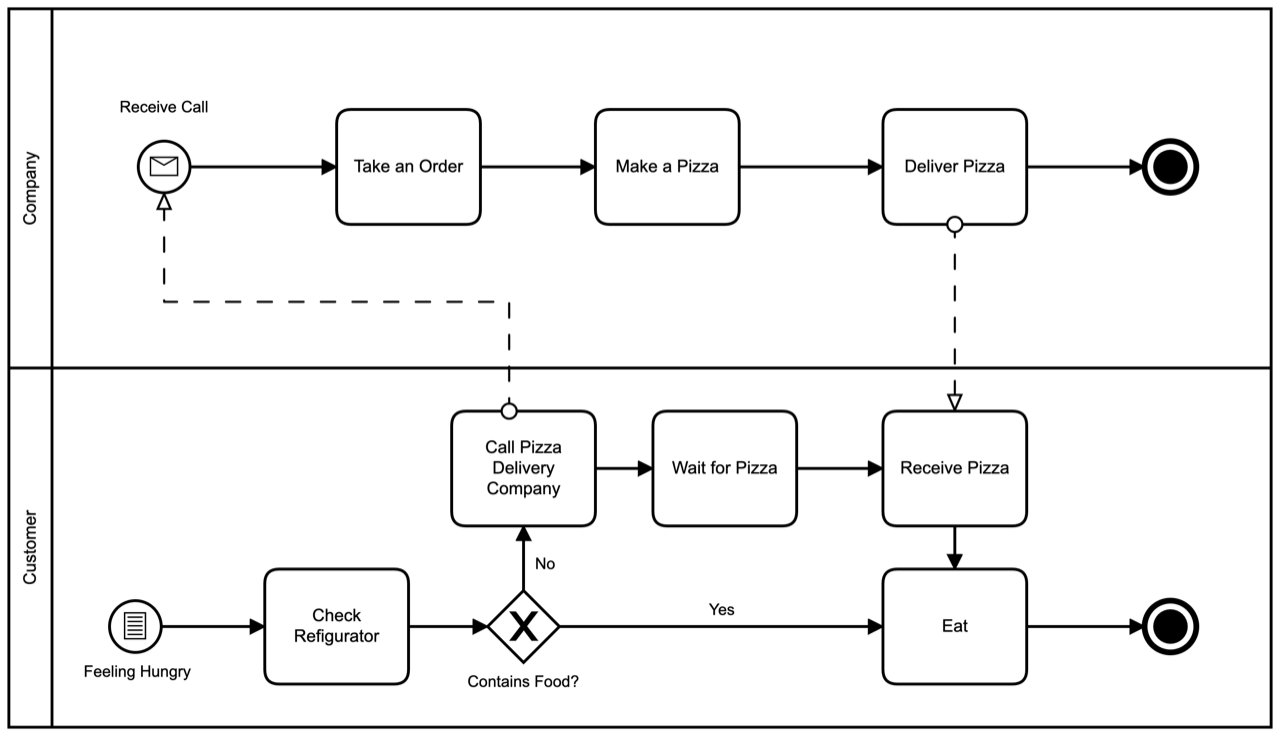
\includegraphics[width=1\textwidth]{PizzaOrder.png}
  \end{center}
  \caption{Example BPMN model for the process of ordering a pizza.}
  \label{fig:length_eight_mouse}
\end{figure}

BPMN is a metamodel used to describe business processes. In its original
version published in 2007 it was only a graphical notation not a full
metamodel as the definition was rather informal and focused mainly on the
visual elements not on the underlying semantics. These gaps were closed with
the release of the BPMN 2.0 specification in 2011 by providing more detailed
information on the semantics of model elements as well as standardized
data-format for BPMN-models based on the XML format.  The BPMN 2.0.1
specification was promoted into an ISO standard in 2013 \cite{iso}.
	
\section{Business Process Definition Metamodel (BPDM)}
The Business Process Metamodel consists of an extensive set of concepts in the
form of language elements. Although this concepts can be used to describe
business processes BPDM does not provide the modeling language to do so. The
fundamental idea is to provide a unified voca\-bulary for other tools and
modeling languages. When implementing such a modeling language one would
define a so called 'mapping' between the created model and BPDM. This enables
translation between different models without changing the meaning of the
portrayed system. Also this would enable platform independence for models as
different software vendors could provide a mapping between their data-format
and BPDM \cite{omg-kol1}.

BPDM consists of different components that focus on different aspects: the
condition model, the composition model and the course model. The
\emph{condition model} defines different ways to represent boolean expressions
and their relation to the real world. The \emph{composition model} describes
concepts that can be used to describe the relation of entities in the real
world. The \emph{course model} contains the concepts to incorporate dynamic
behavior into the models like events and changes over time \cite{bpdm}. The
BPDM definition does not stay completely true to its motivation of being a
metamodel independent of modeling languages but does include some references
to BPMN.

\section{Relevance of BPDM}
Both BPDM and BPMN are maintained by the Object Management Group (OMG). OMG
does also maintain the UML standard. When the original version of BPMN was
published in 2004 it was developed within the Business Process Management
Initiative that in 2005 merged with OMG under the OMG name. In 2006 OMG
released the official BPMN 1.0 standard which did not include a full
metamodel. One year later the vice-president of the OMG organization Jon
Siegel stated that OMG was working on BPDM to provide a metamodel not only for
BPMN but also for all other business process models although BPMN was
specifically considered when designing BPDM. Also BPMN 2.0 was meant to
integrate into BPDM by providing a corresponding mapping and using BPDM
terminology \cite{omg-kol1}. The BPDM specification was published in its final
form in 2008. Three years later in 2011 BPMN 2.0 was released. But instead of
building on BPDM as a metamodel it defines its own metamodel.

In conclusion it is clear that BPDM was mainly created to provide a metamodel
to the already existing BPMN while also providing compatibility to other
modeling languages \cite{blog}. To archive this the metamodel had to be more
complex than otherwise necessary if it would only support BPMN and other
models had to adopt the BPDM. Today there is no wide variety of
modeling languages that adopted BPDM.

\bibliographystyle{unsrt}\raggedright
\begin{thebibliography}{xxx}
\bibitem{blog} Jordi Cabot. \newblock{Has the success of BPMN 2.0 killed
  BPDM}.\\
  \url{https://modeling-languages.com/has-success-bpmn-20-killed-bpdm-business-process-definition-metamodel/},
  November 2010.
\bibitem{bpmn20} Jochen G{\"o}pfert, Heidi Lindenbach.  \newblock {\em
  {Gesch{\"a}ftsprozessmodellierung mit BPMN 2.0}}.  \newblock Oldenbourg
  Wissenschaftsverlag, 2013.
\bibitem{iso} {ISO/IEC Information Technology Task Force}.  \newblock ISO/IEC
  19510:2013, 07/2013.
\bibitem{bpdm} {Object Management Group}.  \emph{Business Process Definition
  MetaModel}. Volume~1, 2008.
\bibitem{BPMN} {Object Management Group}.  \newblock {Business Process Model
  and Notation (BPMN) Version 2.0}, January 2011.
\bibitem{omg-kol1} Jon Siegel.  \newblock {BPDM: Die OMG-Spezifikationen zur
  Gesch{\"a}ftsprozessmodellierung}.  \newblock {\em OBJEKTspektrum}, 2007.
\bibitem{alfwi} Alfred Winter.  \newblock {Vorlesung: Architektur von
  Informationssystemen im Gesundheitswesen}. \newblock Uni Leipzig, 2020.
\end{thebibliography}
%\bibliography{quellen}
\end{document}
